\documentclass[12pt,twoside]{article}
\usepackage{graphicx}
\usepackage{amsmath}
\usepackage{amsfonts}
\usepackage{amssymb}
\usepackage{textcomp}
%\usepackage{subfig}
% \usepackage{wrapfig}
\usepackage{caption}
\usepackage{subcaption}
 
\usepackage[english]{babel}
\usepackage[latin1]{inputenc}
\usepackage[colorlinks,bookmarks=false,linkcolor=blue,urlcolor=blue]{hyperref}

\DeclareMathOperator{\Tr}{Tr}
\newcommand{\mail}[1]{{\href{mailto:#1}{#1}}}
\newcommand{\ftplink}[1]{{\href{ftp://#1}{#1}}}

\begin{document}
\title{Notes on reward function}
\date{\today}
\author{FD}
\maketitle
\begin{abstract}
  Playing around with different definitions for the reward function,
  and keeping track of what is implemented
\end{abstract}

%\tableofcontents

%%%%%%%%%%%%%%%%%%%%%%%%%%%%%%
%%%%%%%%%%%%%%%%%%%%%%%%%%%%%%
\section{Reward function}
We have several different functional forms for the reward function.
Here $x>0$ is the value being optimized, e.g. the
\begin{itemize}
\item A Cauchy distribution
  \begin{equation}
    \label{eq:cauchy-reward}
    f_R(x) = \frac{1}{\pi(1 + x^2)}\,.
  \end{equation}
\item A Gaussian distribution
  \begin{equation}
    \label{eq:gauss-reward}
    f_R(x) = e^{-\tfrac{x^2}{2}}\,.
  \end{equation}
\item An exponential function
  \begin{equation}
    \label{eq:exp-reward}
    f_R(x) = e^{-x}\,.
  \end{equation}
\item The inverse function
  \begin{equation}
    \label{eq:inv-reward}
    f_R(x) = \frac{1}{x+\epsilon}\,.
  \end{equation}
\end{itemize}

\section{Components to the reward}
We consider two components to the reward function: the mass difference
to the target reference, and how soft-wide angle (hard collinear) the
groomed (ungroomed) subjets are.

\subsection{Mass reward}
The mass reward is simply given by
\begin{equation}
  \label{eq:mass-reward}
  R_M(m) = f_R(m - m_\text{target})\,,
\end{equation}
where $m$ is the current mass of the jet.

\subsection{Soft-Drop reward}
The second component to the reward is essentially based on the SD
criterion, and gives a small reward for grooming soft-wide angle
subjets, and for keeping hard-collinear ones.

For groomed jet we want to give a reward if they have
$\ln z,\ln\Delta\sim 0$, while for ungroomed ones, we want to give it
for $\ln z,\ln\Delta \ll 0$.

For the groomed subjet component, we can use a function of the form
\begin{equation}
  \label{eq:groom-rew}
  f_{\text{SD-groom}}(\Delta, z) =
  \min(\exp(\alpha_ 1 \ln(1/\Delta) (-8-\ln z)),1)\,,
\end{equation}
which is shown for $\alpha_1=1$ in figure~\ref{fig:SD-reward-shape}
(left).

For the ungroomed subjets, the function we use is
\begin{equation}
  \label{eq:keep-rew}
  f_{\text{SD-keep}}(\Delta, z) =
  \max(1 - \exp(\alpha_2 \ln(1/\Delta)(-8-\ln z)),0)\,,
\end{equation}
which is shown for $\alpha_2=1/10$ in the right-hand side of
figure~\ref{fig:SD-reward-shape}.

\begin{figure}
  \centering
  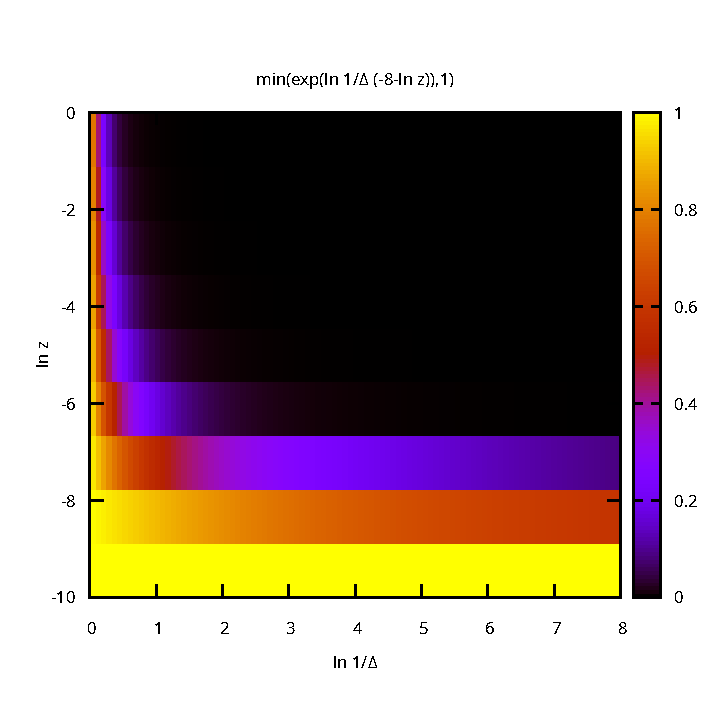
\includegraphics[width=0.5\textwidth,page=1]{SD-reward-test}%
  \includegraphics[width=0.5\textwidth,page=2]{SD-reward-test}%  
  \caption{Shape of the reward function for groomed (left) and ungroomed (right) subjets.}
  \label{fig:SD-reward-shape}
\end{figure}

The Soft Drop component of the reward is then given by
\begin{equation}
  \label{eq:SD-reward}
  R_\text{SD}(\Delta, z) =
  \frac{1}{N}\big[\Theta_{\text{groomed}} f_\text{SD-groom}(\Delta, z)
  + \Theta_\text{ungroomed} f_\text{SD-keep}(\Delta, z)\big]\,.  
\end{equation}
Here $\Theta_\text{groomed}$ is one for groomed subjets and zero
otherwise, $\Theta_\text{ungroomed} = 1 - \Theta_\text{groomed}$, and
$N$ is a normalisation factor suppressing the SD component of the
reward with respect to the mass component.

\subsection{Total reward}

The total reward is simply the sum of equations~(\ref{eq:mass-reward})
and~(\ref{eq:SD-reward}), i.e.
\begin{equation}
  \label{eq:reward}
  R(m,\Delta,z) = R_M(m) + R_\text{SD}(\Delta, z)\,.
\end{equation}

% \begin{thebibliography}{99}
% %\cite{Salam:2009jx}
% \bibitem{Salam:2009jx}
%   G.~P.~Salam,
%   %``Towards Jetography,''
%   Eur.\ Phys.\ J.\ C {\bf 67} (2010) 637
%   [arXiv:0906.1833 [hep-ph]].
%   %%CITATION = ARXIV:0906.1833;%%
%   %185 citations counted in INSPIRE as of 17 Jul 2014
% \end{thebibliography}
\end{document}
